\documentclass[tikz,border=5pt]{standalone}
\usetikzlibrary{arrows.meta,positioning,fit,calc}

\begin{document}
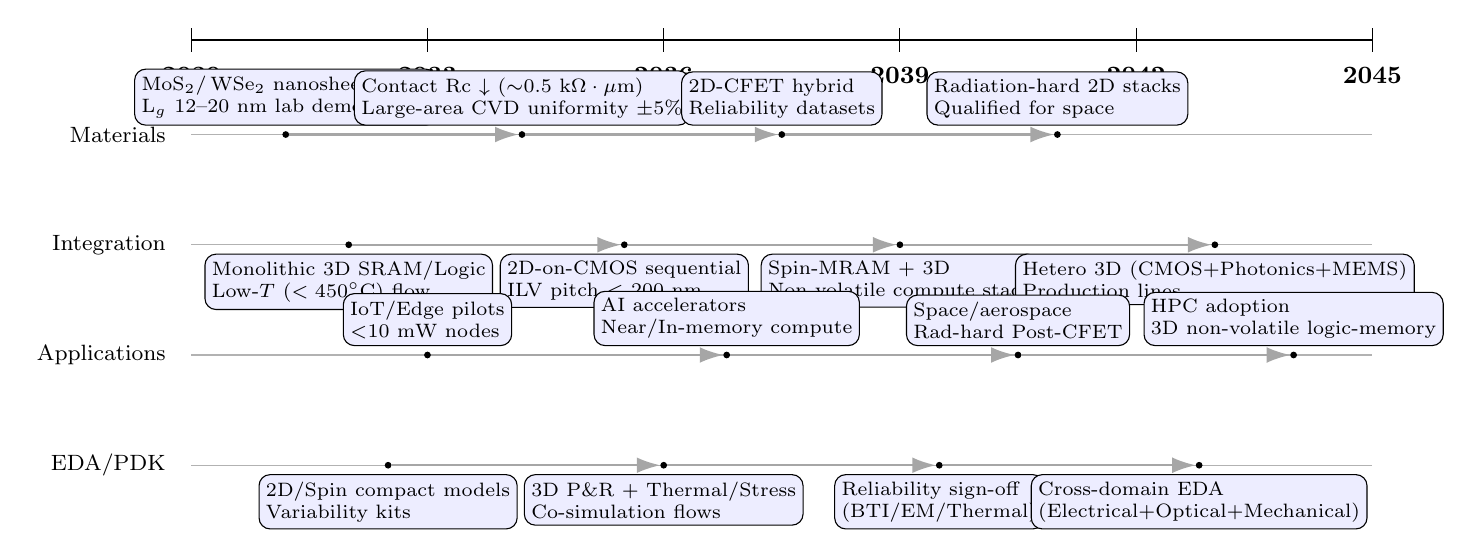
\begin{tikzpicture}[
  >=LaTeX,
  year/.style={font=\bfseries\small},
  lane/.style={font=\footnotesize,align=left},
  bubble/.style={draw, rounded corners, fill=blue!7, align=left, inner sep=2.5pt, font=\scriptsize},
  milestone/.style={circle, draw, fill=black, minimum size=2pt, inner sep=0pt},
  arrow/.style={-{Latex[length=3mm,width=2mm]}, thick}
]
% Axis
\draw[thick] (0,0) -- (15,0);
\foreach \x/\y in {0/2030,3/2033,6/2036,9/2039,12/2042,15/2045} {
  \draw (\x,0.15) -- (\x,-0.15) node[below=2pt,year] {\y};
}

% Lanes
\node[lane, anchor=east] at (-0.2, -1.2) {Materials};
\node[lane, anchor=east] at (-0.2, -2.6) {Integration};
\node[lane, anchor=east] at (-0.2, -4.0) {Applications};
\node[lane, anchor=east] at (-0.2, -5.4) {EDA/PDK};

\draw[gray!60] (0,-1.2) -- (15,-1.2);
\draw[gray!60] (0,-2.6) -- (15,-2.6);
\draw[gray!60] (0,-4.0) -- (15,-4.0);
\draw[gray!60] (0,-5.4) -- (15,-5.4);

% --- Materials lane milestones ---
\node[milestone] (m1) at (1.2,-1.2) {};
\node[bubble, above=2pt of m1] {MoS$_2$/$\,$WSe$_2$ nanosheet FETs \\ L$_g$ 12--20 nm lab demos};
\node[milestone] (m2) at (4.2,-1.2) {};
\node[bubble, above=2pt of m2] {Contact Rc $\downarrow$ ($\sim$0.5 k$\Omega\cdot\mu$m) \\ Large-area CVD uniformity $\pm$5\%};
\node[milestone] (m3) at (7.5,-1.2) {};
\node[bubble, above=2pt of m3] {2D-CFET hybrid \\ Reliability datasets};
\node[milestone] (m4) at (11.0,-1.2) {};
\node[bubble, above=2pt of m4] {Radiation-hard 2D stacks \\ Qualified for space};

% --- Integration lane milestones ---
\node[milestone] (i1) at (2.0,-2.6) {};
\node[bubble, below=2pt of i1] {Monolithic 3D SRAM/Logic \\ Low-$T$ ($<450^\circ$C) flow};
\node[milestone] (i2) at (5.5,-2.6) {};
\node[bubble, below=2pt of i2] {2D-on-CMOS sequential \\ ILV pitch $<$ 200 nm};
\node[milestone] (i3) at (9.0,-2.6) {};
\node[bubble, below=2pt of i3] {Spin-MRAM + 3D \\ Non-volatile compute stack};
\node[milestone] (i4) at (13.0,-2.6) {};
\node[bubble, below=2pt of i4] {Hetero 3D (CMOS+Photonics+MEMS) \\ Production lines};

% --- Applications lane milestones ---
\node[milestone] (a1) at (3.0,-4.0) {};
\node[bubble, above=2pt of a1] {IoT/Edge pilots \\ $<$10 mW nodes};
\node[milestone] (a2) at (6.8,-4.0) {};
\node[bubble, above=2pt of a2] {AI accelerators \\ Near/In-memory compute};
\node[milestone] (a3) at (10.5,-4.0) {};
\node[bubble, above=2pt of a3] {Space/aerospace \\ Rad-hard Post-CFET};
\node[milestone] (a4) at (14.0,-4.0) {};
\node[bubble, above=2pt of a4] {HPC adoption \\ 3D non-volatile logic-memory};

% --- EDA/PDK lane milestones ---
\node[milestone] (e1) at (2.5,-5.4) {};
\node[bubble, below=2pt of e1] {2D/Spin compact models \\ Variability kits};
\node[milestone] (e2) at (6.0,-5.4) {};
\node[bubble, below=2pt of e2] {3D P\&R + Thermal/Stress \\ Co-simulation flows};
\node[milestone] (e3) at (9.5,-5.4) {};
\node[bubble, below=2pt of e3] {Reliability sign-off \\ (BTI/EM/Thermal)};
\node[milestone] (e4) at (12.8,-5.4) {};
\node[bubble, below=2pt of e4] {Cross-domain EDA \\ (Electrical+Optical+Mechanical)};

% Arrows indicating progression
\draw[arrow, gray!70] (m1) -- (m2);
\draw[arrow, gray!70] (m2) -- (m3);
\draw[arrow, gray!70] (m3) -- (m4);

\draw[arrow, gray!70] (i1) -- (i2);
\draw[arrow, gray!70] (i2) -- (i3);
\draw[arrow, gray!70] (i3) -- (i4);

\draw[arrow, gray!70] (a1) -- (a2);
\draw[arrow, gray!70] (a2) -- (a3);
\draw[arrow, gray!70] (a3) -- (a4);

\draw[arrow, gray!70] (e1) -- (e2);
\draw[arrow, gray!70] (e2) -- (e3);
\draw[arrow, gray!70] (e3) -- (e4);

\end{tikzpicture}
\end{document}